\documentclass{exam} 
\printanswers 
\def\workshopTitle{Workshop - Workshop - Classes and Objects 1, JUnit} 
\input{comp125workshopHeader}\section*{Learning outcomes}

By the end of this session, you will know some of Java basics.
In particular, you will be able to design and write simple Java classes.

\section*{Questions}

\begin{questions}

\question {\bf Import-Export}\\
 
It is important to know how to import Java projects from archive files (.jar/ .zip).

For this exercise, download the file \texttt{week3.zip} from iLearn but \color{red}DO NOT unzip/open it\color{black}.

\begin{enumerate}
\item Click "File" --> "Import" --> "Existing Projects into Workspace" \color{red}\textbf{and NOT "Archive file"}\color{black}.
\item Select option "Select Archive file" and click on "Browse"
\item Choose the archive file ("week3.zip") that contains project(s) you want to open. Please note an archive file may contain multiple projects and click "ok"
\item Check all projects you want to import
\item Click "Finish"
\end{enumerate}

You should see a project \texttt{week3workshop} if correctly imported.

%Next, we'll learn how to export a project.
%
%\begin{enumerate}
%\item Click ``File" --> ``Export" --> ``General" --> ``Archive file"
%\item Select all projects you want to export in the archive file in the left panel
%\item In the ``To archive file" section, choose file path and name
%\item Click ``Finish"
%\end{enumerate}
%
%Export the project \texttt{classesAndObjects} to an archive file \texttt{exported.zip}.

\newpage
\question Design classes (no implementation) that encapsulate the following real life entities. Add up to three instance variables for each class. Select the three most important attributes if you think a class has more than three attributes. Describe your design in terms of a UML class diagram as shown in the lecture.

\begin{enumerate}
\item \texttt{Person}
\item \texttt{Cylinder}
\item \texttt{Book} \textbf{(Take-home exercise)}
\end{enumerate}

\begin{solution}
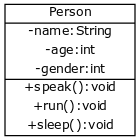
\includegraphics[width=5cm]{Person.png}
\vskip 0.5cm
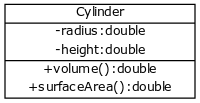
\includegraphics[width=5cm]{Cylinder.png}
\vskip 0.5cm
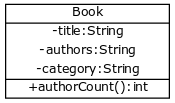
\includegraphics[width=5cm]{Book.png}
\vskip 0.5cm
\end{solution}

\question 

\begin{parts}

\part Consider the following class definition,

\begin{lstlisting}
public class Date {
	public int day, month, year;
}
\end{lstlisting}

In a client code (outside the class \texttt{Date}), create an object to represent 13th April, 2011.

\begin{solution}
\begin{lstlisting}
Date graduation = new Date();
graduation.day = 13;
graduation.month = 4;
graduation.year = 2011;
\end{lstlisting}
\end{solution}

\part For the same class definition (\texttt{Date}), draw the memory diagram that represents the following objects. Please refer to the lecture notes to see the representation scheme we have established.

\begin{lstlisting}
Date bday = new Date();
bday.day = 31;
bday.month = 7;
bday.year = 1980;

Date anniversary = null;
\end{lstlisting}

\begin{solution}
\begin{tikzpicture}
\memoryblock{width=2, height=1, array={"bday"}}
\arrow{startX=1.6, startY=0.5, endX=5, endY=0.5}
\memoryblock{x=5, y=-2, width=3, height=3, array={"day = 31", "month = 7", "year = 1980"}}
\end{tikzpicture}

\begin{tikzpicture}
\memoryblock{width=4, height=1, array={"anniversary = null"}}
\end{tikzpicture}
\end{solution}

\part \textbf{(Take-home exercise)} Consider the following class definition,

\begin{lstlisting}
public class Car {
	public String model;
	public int price;
}
\end{lstlisting}

In a client code (outside the class \texttt{Car}), create an object to represent a Toyota Corolla priced at \$21,999.

\begin{solution}
\begin{lstlisting}
Car myCar = new Car();
myCar.model = "Toyota Corolla";
myCar.price = 21999;
\end{lstlisting}
\end{solution}
\end{parts}
\newpage

\question 
\begin{parts}

\part Consider the following class definition,

\begin{lstlisting}[frame=single,style=buggy]
public class Person {
	public String name;
	public int age;
}
\end{lstlisting}

With the help of an example, explain why it's a bad idea for the instance variables to be public.

\begin{solution}
\begin{lstlisting}
Person p = new Person();
p.name = "Hagrid";
p.age = -6; //OOPS!
\end{lstlisting}
\end{solution}

\part Solve the problem of \texttt{public} instance variables in the previous part by first changing visibility of the instance variables of class \texttt{Person} to \texttt{private} and then adding getters and setters. Age of a person cannot be negative. If the user tries to assign a negative value to a person's age, the person's age should be set to 0.


\begin{solution}
\begin{lstlisting}
public class Person {
	private String name;
	private int age;

	//setters
	public void setName(String str) {
		name = str;
	}
	
	public void setAge(int a) {
		if(a <= 0)
			age = 0;
		else
			age = a;
	}
	
	public String getName() {
		return name;
	}

	public int getAge() {
		return age;
	}
}
\end{lstlisting}
\end{solution}

\part Declare and instantiate an object \texttt{baddy} of class \texttt{Person} written in the previous part, representing a person named "Tom Marvolo Riddle" aged 71.

\begin{solution}
\begin{lstlisting}
Person baddy = new Person();
baddy.setName("Tom Marvolo Riddle");
baddy.setAge(71);
\end{lstlisting}
\end{solution}

\part Declare and instantiate an object \texttt{goody} of class \texttt{Person} written in the previous part, representing a person named "Luna Lovegood". Try and assign the value -6 to her age. Display the values of the instance variables on the console.

\begin{solution}
\begin{lstlisting}
Person goody = new Person();
goody.setName("Luna Lovegood");
goody.setAge(6);
System.out.println(goody.getName()); //"Luna Lovegood"
System.out.println(goody.getAge()); //0
\end{lstlisting}
\end{solution}

\part List the mistakes (syntactical and logical) in the following constructor for class \texttt{Person} - 

\begin{lstlisting}
public void person(String s, int a) {
	name = s;
	age = a;
}
\end{lstlisting}

\begin{solution}
\begin{itemize}
\item Constructor should have no return type, not even void.
\item Name of constructor should be \textbf{exactly} the same as the class name. So, \texttt{Person}, not \texttt{person}.
\item Constructor should use setters to assign values to instance variables.
\end{itemize}

Fixed constructor,

\begin{lstlisting}
public Person(String s, int a) {
	setName(s);
	setAge(a);
}
\end{lstlisting}
\end{solution}

\part Add a constructor to class \texttt{Person} with a single parameter for the instance variable name. The instance variable \texttt{age} should be set to 21.

\begin{solution}
\begin{lstlisting}
public Person(String s) {
	setName(s);
	setAge(18); //setter is used here as a best practice.
}
\end{lstlisting}
\end{solution}

\part Assuming the constructor have been added to class \texttt{Person} according to previous part. Will the following program run successfully, or result in a compilation error? Explain your answer. Also, if there is a compilation error, what should be done to fix it?

\begin{lstlisting}
Person p = new Person();
\end{lstlisting}

\begin{solution}
It will result in a compilation error, since once parameterized constructors are defined, Java expects us to define the default constructor as well, and the default constructor that Java provides is no longer valid. The solution, therefore, is to add a default constructor.

\begin{lstlisting}
public Person() {
	setName("anonymous");
	setAge(0);
}
\end{lstlisting}
\end{solution}
\end{parts}

\vskip 0.5cm

\question {\bf JUnit Testing}\\

We can test the correctness of individual methods through running JUnit tests on them. 

In the project that you imported, open file \texttt{RectangleTest.java} and run it. You will see a green bar and a message that 5 out of 5 tests have passed (0 errors and 0 failures).

Now open the file \texttt{AllInOneTest.java} and run the tests. You will see that two tests pass while one fails. The tests that pass are:

\begin{enumerate}
  \item \texttt{testIsSquare}: This tests the method \texttt{isSquare} from class \texttt{AllInOne}
  \item \texttt{testAllSquares}: This tests the method \texttt{allSquares} from class \texttt{AllInOne}
\end{enumerate}

The test that fails is \texttt{testCountPositiveEvens}: This tests the method \texttt{countPositiveEvens} from class \texttt{AllInOne}. 

Your job is to complete the method \texttt{countPositiveEvens} so the test \texttt{testCountPositiveEvens} passes. \textbf{IMPORTANT: } note that the method should return 0 if the array passed is \texttt{null}. This is the first thing you should check in the method. 

\begin{solution}
Refer to project in Eclipse archive file week3solution.zip	
\end{solution}

\vskip 0.5cm

\question {\bf compareTo method}\\

Consider the class \texttt{GoalScoringRecord} in the project imported. Complete the method \texttt{compareTo} so the corresponding test supplied in class \texttt{GoalScoringRecordTest} passes.

\begin{solution}
Refer to project in Eclipse archive file week3solution.zip	
\end{solution}

%\newpage
%
%\question {\bf Take-home Programming Exercise}\\
%
%\begin{enumerate}
%\item Write a class definition for a \texttt{Cylinder}, as represented by its radius and height. It should include,
%
%\begin{enumerate}
%\item Correct class header.
%\item instance variables with appropriate visibility and data types.
%\item Getters
%\item Setters, with appropriate validation.
%\item Constructors
%	\begin{enumerate}
%		\item With no parameters. Set each instance variable to 1.
%		\item With two parameters, one for each instance variable.
%	\end{enumerate}
%\item A method \texttt{volume()} that returns the volume of the cylinder. The formula for volume of a cylinder with radius $r$ and height $h$ is $\pi \times r^2 \times h$ (where $r$ is the radius of the circle). The value of $\pi$ in Java is given by \texttt{Math.PI}, and square of a number $n$ is calculated as \texttt{n*n} or \texttt{Math.pow(n,2)}, and \textcolor{red}{NOT \problem{n\^{}2} or \problem{Math.sqr(n)}}.
%\end{enumerate}
%
%\item Create a Client \texttt{CylinderClient} that performs the following tasks -
%
%	\begin{enumerate}
%	\item Create a \texttt{Cylinder} object \texttt{c1} that has a radius of 2.5 and height of 4.7
%	\item Display the volume of \texttt{c1}.
%	\item Increase the radius of \texttt{c1} by 2.1
%	\item Display the volume of \texttt{c1}.
%	\end{enumerate}
%	
%\end{enumerate}
%\begin{solution}
%\newpage
%
%Cylinder.java
%\begin{lstlisting}
%public class Cylinder {
%	private double radius, height;
%	
%	public void setRadius(double r) {
%		radius = Math.abs(r);
%	}
%	
%	public void setHeight(double h) {
%		height = Math.abs(h);
%	}
%	
%	public double getRadius() {
%		return radius;
%	}
%	
%	public double getHeight() {
%		return height;
%	}
%	
%	public Cylinder() {
%		setRadius(1);
%		setHeight(1);
%	}
%	
%	public Cylinder(double r, double h) {
%		setRadius(r);
%		setHeight(h);
%	}
%	
%	public double volume() {
%		return Math.PI * radius * radius * height;
%	}		
%}
%\end{lstlisting}
%
%CylinderClient.java
%\begin{lstlisting}
%public class CylinderClient {
%	public static void main(String[] args) {
%		Cylinder c1 = new Cylinder(2.5, 4.7);
%		System.out.println(c1.area());
%		c1.setRadius(c1.getRadius() + 2);
%		System.out.println(c1.area());
%	}
%}
%\end{lstlisting}
%\end{solution}

\end{questions}


\end{document}
